% Copyright 2004 by Till Tantau <tantau@users.sourceforge.net>.
%
% In principle, this file can be redistributed and/or modified under
% the terms of the GNU Public License, version 2.
%
% However, this file is supposed to be a template to be modified
% for your own needs. For this reason, if you use this file as a
% template and not specifically distribute it as part of a another
% package/program, I grant the extra permission to freely copy and
% modify this file as you see fit and even to delete this copyright
% notice. 

\documentclass{beamer}
\usepackage{amsmath,amsfonts,amssymb,amsthm}
\usepackage{eqparbox}
\usepackage{textcomp}
\usepackage{blindtext}
\usepackage{textgreek}
\usepackage{gensymb}
\usepackage{xcolor}
\usepackage{color}
\usepackage{soul}
\usepackage{placeins}
\usepackage{graphics}
\usepackage{graphicx}
\usepackage{textpos}
\usepackage{caption}
\usepackage{color}
\usepackage{bm}
\usepackage{tikz}
\usepackage{pgf}
\captionsetup[figure]{labelformat=empty}
\graphicspath{{Figures/}}
\usepackage[natbib=true, style=numeric, sorting=none, backend=bibtex]{biblatex}
\addbibresource{MastersSeminarUpdated.bib}

% There are many different themes available for Beamer. A comprehensive
% list with examples is given here:
% http://deic.uab.es/~iblanes/beamer_gallery/index_by_theme.html
% You can uncomment the themes below if you would like to use a different
% one:
%\usetheme{AnnArbor}
%\usetheme{Antibes}
%\usetheme{Bergen}
%\usetheme{Berkeley}
%\usetheme{Berlin}
%\usetheme{Boadilla}
%\usetheme{boxes}
%\usetheme{CambridgeUS}
\usetheme{Copenhagen}
%\usetheme{Darmstadt}
%\usetheme{default}
%\usetheme{Frankfurt}
%\usetheme{Goettingen}
%\usetheme{Hannover}
%\usetheme{Ilmenau}
%\usetheme{JuanLesPins}
%\usetheme{Luebeck}
%\usetheme{Madrid}
%\usetheme{Malmoe}
%\usetheme{Marburg}
%\usetheme{Montpellier}
%\usetheme{PaloAlto}
%\usetheme{Pittsburgh}
%\usetheme[height=10mm]{Rochester}
%\usetheme{Singapore}
%\usetheme{Szeged}
%\usetheme{Warsaw}

%\useoutertheme[footline=authortitle]{miniframes}
\usecolortheme{default}

\title{Determination of Hardness Factors for Various Proton Beams}

% A subtitle is optional and this may be deleted
%\subtitle{Cameron Simpson-Allsop}

\author{C. Simpson-Allsop, L. Ram, K. Nikolopoulos, T. Price, I. Mateu \vspace{-1cm}}
% - Give the names in the same order as the appear in the paper.
% - Use the \inst{?} command only if the authors have different
%   affiliation.
\date{University of Birmingham, \\ \vspace{0.1cm} \today}
% - Either use conference name or its abbreviation.
% - Not really informative to the audience, more for people (including
%   yourself) who are reading the slides online

% If you have a file called "university-logo-filename.xxx", where xxx
% is a graphic format that can be processed by latex or pdflatex,
% resp., then you can add a logo as follows:

% \pgfdeclareimage[height = 1cm]{logo}{Figures/UoB_logo.png}
% \logo{\pgfuseimage{logo}}
 
\titlegraphic{\includegraphics[width=1.5cm]{UoB_logo.png}\hspace*{4.75cm}~%
   \includegraphics[width=1.5cm]{ATLAS_logo.png}
}

\addtobeamertemplate{navigation symbols}{}{%
    \usebeamerfont{footline}%
    \usebeamercolor[fg]{footline}%
    \hspace{1em}%
    \insertframenumber/\inserttotalframenumber
}

\begin{document}

\begin{frame}
  \titlepage
\end{frame}

\begin{frame}{Outline}
    \begin{enumerate}
        \item Introduction
        \vspace{0.5cm}
        \item Other Studies and Current Values
        \vspace{0.5cm}
        \item I--V Measurements
        \vspace{0.5cm}
        \item C--V Measurements
        \vspace{0.5cm}
        \item Irradiations using the MC40 Cyclotron
        \vspace{0.5cm}
        \item Determination of Hardness Factors
        \vspace{0.5cm}
        \item Conclusion and Outlook
    \end{enumerate}
\end{frame}

\begin{frame}{Introduction}
 Utilizing the \textbf{I--V} and \textbf{C--V} characteristics of \textbf{BPW34F photodiodes}, the \textbf{Hardness Factors}, $\kappa$, of three different proton beams have been measured.
  \vspace{0.3cm}
  \begin{itemize}
  \item The \textbf{MC40 Cyclotron} at the \textbf{University of Birmingham} (25 MeV).
  \vspace{0.1cm}
  \item The \textbf{IRRAD Proton Facility} at \textbf{CERN} (24 GeV).
  \vspace{0.1cm}
  \item The \textbf{Irradiations Facility} at the \textbf{Karlsruhe Institute of Technology} (24 MeV).
  \end{itemize}
  \vspace{0.3cm}
 For \textbf{IRRAD}, the Results were compared to a similar study undertaken by \textbf{I. Mateu} this year.
\end{frame}

\begin{frame}{Other Studies and Current Values}
\begin{itemize}
    \item Current \textbf{MC40 cyclotron} value: \textbf{2.2} for \textbf{25 MeV protons} \textsuperscript{\cite{krakow}}.
    \vspace{0.5cm}
    \item \textbf{KIT}: \bm{$2.05 \pm 0.61$} for \textbf{24 MeV protons}, with a previous assumption of \textbf{1.85} for \textbf{26 MeV protons} \textsuperscript{\cite{Karlsruhe}}.
    \vspace{0.5cm}
    \item \textbf{Tabulated values} from RD50: \bm{$\sim 2.56$} for \textbf{25 MeV protons} \textsuperscript{\cite{RD50}}.
    \vspace{0.5cm}
    \item Studies at the \textbf{IRRAD facility}: \textbf{0.56} (2015), and \textbf{0.60} (2016) for \textbf{24 GeV protons} \textsuperscript{\cite{IRRAD}}. 
\end{itemize}
    
\end{frame}

    \begin{frame}{I--V Measurements}{Setup}
        \begin{minipage}{0.6\linewidth}
        \begin{figure}
            \centering
            \includegraphics[width = \linewidth]{IV_Setup.jpg}
            \caption{Experimental setup for I--V measurements.}
        \end{figure}
        \end{minipage}%
        \begin{minipage}{0.4\linewidth}
            \begin{itemize}
                \item Aluminium shielded box containing the photodiode.
                \item Keithley 2410 Source Meter for I--V measurements of the photodiode.
                \item Thermocouple to monitor temperature.
                \item Power supply for a fan within the box.
            \end{itemize}
        \end{minipage}
    \end{frame}
    
    \begin{frame}{I--V Measurements}{Setup}
        \begin{minipage}{0.6\linewidth}
        \begin{figure}
            \centering
            \includegraphics[width = \linewidth]{Photodiode_Box.jpg}
            \caption{Aluminium shielding box.}
        \end{figure}
        \end{minipage}%
        \begin{minipage}{0.4\linewidth}
        \begin{itemize}
            \item Thermocouple fixed close to the photodiode.
            \item Electric fan for air circulation.
            \item Tape across any gaps in the box to block out light.
            \item The lid of the box could be closed to shield the system in Aluminium.
        \end{itemize}
        \end{minipage}
    \end{frame}
    
    \begin{frame}{C--V Measurements}{Current -- Voltage Relation and Maximum Depletion Voltage.}
        \begin{itemize}
            \item The \textbf{capacitance} of a photodiode is related to the \textbf{reverse bias} by \textsuperscript{\cite{Casse}}:
                \begin{equation*}
                    C = \frac{f\sqrt{\epsilon_{Si}\epsilon_0}}{\sqrt{V}}
                \end{equation*}
            \item At \textbf{maximum depletion voltage}, capacitance becomes independent of voltage.
            \vspace{0.5cm}
            \item Plotting \textbf{capacitance vs voltage} on a log plot should therefore show a straight line, with a \textbf{deviation} at maximum depletion.
        \end{itemize}
    \end{frame}
    
    \begin{frame}{C--V Measurements}{Setup}
        \begin{minipage}{0.55\linewidth}
        \begin{figure}
            \centering
            \includegraphics[width = \linewidth]{CVSetup.jpg}
            \caption{Experimental setup for C--V measurements.}
        \end{figure}
        \end{minipage}%
        \begin{minipage}{0.45\linewidth}
        \begin{itemize}
            \item Keithley 2410 Source Meter, Wayne Kerr Component Analyser and photodiode setup connected to a junction box.
            \item Keithley used to apply bias across the photodiode.
            \item Wayne Kerr used to measure capacitance across the photodiode at the bias set by the Keithley.
        \end{itemize}
        \end{minipage}
    \end{frame}
    
    \begin{frame}{C--V Measurements}{Calculating Maximum Depletion Voltage}
        \begin{itemize}
            \item By calculating the \textbf{intersect} of the two fits, the point at which the trend deviates from a straight line could be calculated.
            \vspace{0.3cm}
            \item Applying this method, a maximum depletion voltage value of $\bm{V_{dep} = -90.8 \pm 0.22}$ \textbf{V} was inferred. 
        \end{itemize}
        \begin{figure}
            \centering
            \includegraphics[width = 0.7\linewidth]{Diode2_nonirradiated_CV_noextrapolation_1711.pdf}
            \vspace{-0.4cm}
            \caption{log capacitance vs log voltage.}
            \label{fig:CVNonIrradiated}
        \end{figure}
    \end{frame}
    
    \begin{frame}{Proton Irradiations}{ATLAS Chamber}
        \begin{figure}
            \begin{minipage}[b]{0.5\linewidth}
            \centering
            \includegraphics[width = 0.98\textwidth]{ATLAS_chamber.jpg}
        \end{minipage}%
        \begin{minipage}[b]{0.5\linewidth}
            \centering
            \includegraphics[width = 0.98\textwidth]{Isolation_box.jpg}
        \end{minipage}
        \end{figure}
        The environmental chamber at the MC40 high intensity irradiation facility. The photodiodes were installed in the chamber using dedicated aluminium mounts, and then irradiated at $-27^{\circ}$C.
    \end{frame}

    \begin{frame}{Proton Irradiations}{Mounting the Photodiodes}
        \centering
        $\otimes$ Beam direction.
        \begin{figure}
            \begin{minipage}[b]{0.5\linewidth}
            \centering
            \includegraphics[width = 0.98\textwidth]{Mount_no_Foils.jpg}
        \end{minipage}%
        \begin{minipage}[b]{0.5\linewidth}
            \centering
            \includegraphics[width = 0.98\textwidth]{Mount_with_Foils.jpg}
        \end{minipage}
        \end{figure}
        \centering
        Aluminium mount. The nickel foils were used to measure the incident fluence.
    \end{frame}

    \begin{frame}{Computing Hardness Factors}{Leakage Current Variation with Fluence}
        \begin{itemize}
            \item Post irradiation, all photodiodes were annealed for 80 minutes at 60\degree C.
            \item The \textbf{change in leakage current} before and after irradiation is related to \textbf{proton fluence} by \textsuperscript{\cite{Moll}}:
                \begin{equation*}
                    \Delta I = \alpha L^2 w \phi
                \end{equation*}
            \item The \textbf{hardness factor} can be written as:
                \begin{equation*}
                    \kappa = \frac{\alpha}{\alpha _{neq}}\hspace{0.5cm}\text{since}\hspace{0.5cm}\kappa = \frac{\phi _{neq}}{\phi}
                \end{equation*}
                Where $\alpha _{neq} = (3.99 \pm 0.03)\times 10^{-17}$ Acm\textsuperscript{-1} \textsuperscript{\cite{Moll}}.
        \end{itemize}
    \end{frame}
    
    \begin{frame}{Results}{Hardness Factor of the MC40 Cyclotron}
        \begin{figure}
            \centering
            \includegraphics[width = 0.9\linewidth]{MC40_seminar.pdf}
        \end{figure}
    \vspace{-0.3cm}
    From this, a value of \bm{$\kappa _{MC40} = 2.20 \pm 0.08$} for \textbf{25 MeV protons} was inferred. These data were obtained with BPW34F photodiodes.
    \end{frame}

    \begin{frame}{Results}{Hardness Factor of the IRRAD Proton Facility}
        \begin{figure}
            \centering
            \includegraphics[width = 0.9\linewidth]{IRRAD_seminar.pdf}
        \end{figure}
    Using the same method as for the MC40 Cyclotron, a value of \bm{$\kappa _{IRRAD} = 0.62 \pm 0.02$} for \textbf{24 GeV protons} was inferred. These data were also obtained with BPW34F photodiodes.
    \end{frame}
    
    \begin{frame}{Results}{Hardness Factor of the IRRAD Proton Facility - Comparison with I. Mateu's Data}
        \begin{figure}
            \centering
            \includegraphics[width = 0.9\linewidth]{Isidre_seminar.pdf}
        \end{figure}
    \vspace{-0.5cm}
    Analysis of I. Mateu's data yields a value of \bm{$\kappa _{Mateu} = 0.62 \pm 0.02$} with all points included, which is in agreement with his own analysis and our result. These data were obtained with FZ pad diodes.
    \end{frame}
    
    \begin{frame}{Results}{Hardness Factor of the IRRAD Proton Facility - Comparison with I. Mateu's Data}
    For I. Mateu's data, the maximum depletion voltage was calculated for each sensor, and so was not kept constant across all data points.
        \begin{figure}
            \centering
            \includegraphics[width = 0.9\linewidth]{IsidreCVexample.pdf}
            \caption{Example $\frac{1}{C^2}$ --V curve for I. Mateu's data analysis.}
        \end{figure}
    \end{frame}
    
    \begin{frame}{Results}{Hardness Factor of the IRRAD Proton Facility - Comparison with I. Mateu's Data}
    \begin{table}[htb]
        \centering
        \begin{tabular}{|c|c|c|}
            \hline
            Sensor Name & Max. Dep. Voltage (-V) & Fluence (p/cm\textsuperscript{2}) \\
            \hline
            W332-C4 & $249.52\pm 0.09$ & $7.44\times 10^{12}$\\
            W332-F2 & $83.13\pm 0.52$ & $9.66 \times 10^{13}$\\
            W332-F8 & $190.97\pm 1.44$ & $2.41\times 10^{13}$\\
            W332-M10 & $281.09\pm 0.13$ & $1.09\times 10^{12}$\\
            W332-M12 & $80.74\pm 0.35$ & $9.66\times 10^{13}$\\
            W332-M4 & $281.68\pm 0.13$ & $1.09\times 10^{12}$\\
            W332-M6 & $207.36\pm 0.89$ & $2.41\times 10^{13}$\\
            W332-M7 & $252.41\pm 0.15$ & $7.44\times 10^{12}$\\
            \hline
        \end{tabular}
        \caption{Obtained maximum depletion voltages for I. Mateu's data.}
    \end{table}
    \end{frame}
    
    \begin{frame}{Hardness Factor of the KIT Irradiations Facility}
        \begin{figure}
            \centering
            \includegraphics[width = 0.8\linewidth]{KIT_seminar.pdf}
        \end{figure}
    The highest fluence point was ignored to omit the non-linearity region ($\sim 10^{13}$ n\textsubscript{eq}/cm\textsuperscript{2} \textsuperscript{\cite{Ravotti}}). This gave a value of \bm{$\kappa _{KIT} = 2.20 \pm 0.28$} for \textbf{24 MeV protons}. These data were obtained with BPW34F photodiodes.    
    \end{frame}
    
\begin{frame}{Conclusion and Outlook}
  \begin{itemize}
  \item The I--V and C--V characteristics of BPW34F photodiodes have been analysed.
  \vspace{0.3cm}
  \item Using these characteristics, hardness factors for various proton beams have been determined.
  \vspace{0.3cm}
  \item The results are in good agreement with other studies.
  \vspace{0.3cm}
  \item In the future, it is suggested that studies are done to determine the current related damage rate for neutrons (This study assumed a value of $\alpha _{neq} = (3.99 \pm 0.03)\times 10^{-17}$ Acm\textsuperscript{-1} \textsuperscript{\cite{Moll}}), and therefore, determine independent hardness factor values.
  \end{itemize}    
\end{frame}

\begin{frame}[allowframebreaks]{References}
    \printbibliography[heading=none]
\end{frame}

\begin{frame}{Extra Slides}{Fluence Determination}
        \begin{minipage}{0.45\linewidth}
            \begin{figure}
                \centering
                \includegraphics[width = 0.9\linewidth, trim = {6.5cm 11.5cm 5.5cm 2cm}, clip = true]{Counter.pdf}
                \caption{\footnotesize Schematic diagram of germanium counter.}
            \end{figure}
        \end{minipage}%
        \begin{minipage}{0.55\linewidth}
            \begin{itemize}
                \item The \textbf{irradiated nickel foils} were analyzed using a \textbf{germanium counter}.
                \item Due to the weak activity of the foils, they had to be placed directly on top of the counter.
                \item A \textbf{ratio of counts} was taken between this position and the calibrated position.
                \item The measured counts from the foils were then converted into \textbf{proton fluences}.
            \end{itemize}
        \end{minipage}%        
\end{frame}

\begin{frame}{Extra Slides}{Beam Energy Determination}
    \begin{figure}
        \centering
        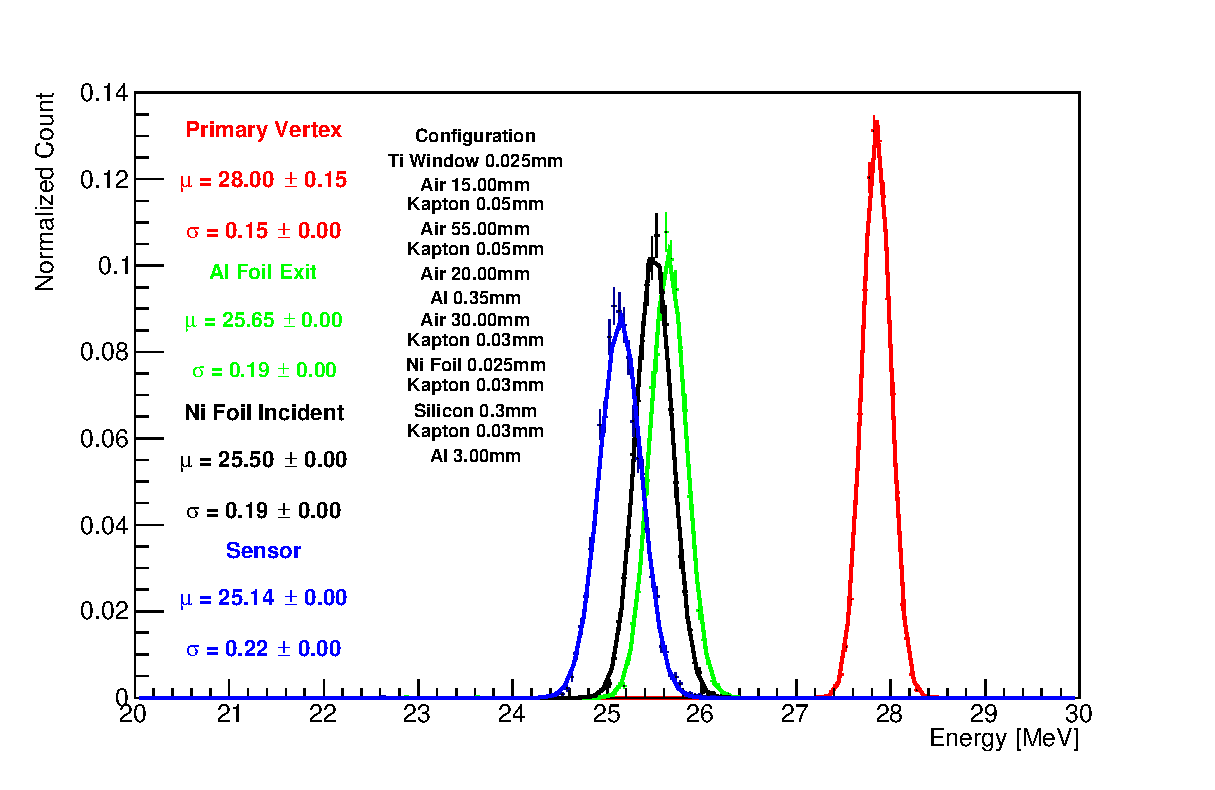
\includegraphics[width = 0.8\linewidth]{28MeV_incidentEnergy.eps}
        \caption{Geant4 simulation revealing the incident beam energy, the energy at the nickel foils, and the energy at the sample (Courtesy of Dr. T. Price).}
    \end{figure}
\end{frame}

\end{document}
